% docs/.paper/sec_method.tex
\section{Problem Formulation \& Methodology}
\label{sec:method}

This section defines the repository translation problem, describes the system architecture of MAgHARCM, and details the four cooperating agents in our pipeline.

\subsection{Problem Formulation}
\label{sec:method_formulation}

We define repository-scale translation as a structured mapping between source and target software projects. A source project is defined as:
\begin{equation}
P_s = (F_s, T_s, D_s, \mathcal{M}_s)
\end{equation}
where $F_s = \{f_1, f_2, \dots, f_n\}$ is the set of source code files in language $L_s$, $T_s = \{t_1, t_2, \dots, t_m\}$ is the test suite, $D_s$ represents library dependencies from the build manifest, and $\mathcal{M}_s$ defines the module directory structure.

The objective is to synthesize a target project:
\begin{equation}
P_t = (F_t, T_t, D_t, \mathcal{M}_t)
\end{equation}
in target language $L_t$ (such as Rust) satisfying three conditions:
\begin{enumerate}
    \item \textbf{Syntactic and Type Compilation Validity ($\mathcal{C}$):} The target project $P_t$ compiles cleanly under target compiler toolchain $\mathcal{T}_{L_t}$ with zero errors:
    \begin{equation}
    \mathcal{C}(P_t) = \text{Compile}(\mathcal{T}_{L_t}, P_t) = \text{True}
    \end{equation}
    \item \textbf{Observational Semantic Equivalence ($\mathcal{E}$):} For every source function $u_s \in F_s$ and translated target function $u_t \in F_t$, execution outputs must match for all valid inputs $x \in I$:
    \begin{equation}
    \forall x \in I, \quad \text{Exec}(u_s, x) \equiv \text{Exec}(u_t, x)
    \end{equation}
    \item \textbf{Test Suite Verification \& Assertion Integrity ($\mathcal{V}$):} The translated test suite $T_t$ must pass completely while preserving all test assertions from $T_s$:
    \begin{equation}
    \begin{aligned}
    \mathcal{V}(T_t, P_t) = &\left( \text{TestPassRate}(T_t) = 1.0 \right) \ \land \\
    &\left( \text{AssertCount}(T_t) \ge \text{AssertCount}(T_s) \right)
    \end{aligned}
    \end{equation}
\end{enumerate}

\begin{figure*}[!t]
    \centering
    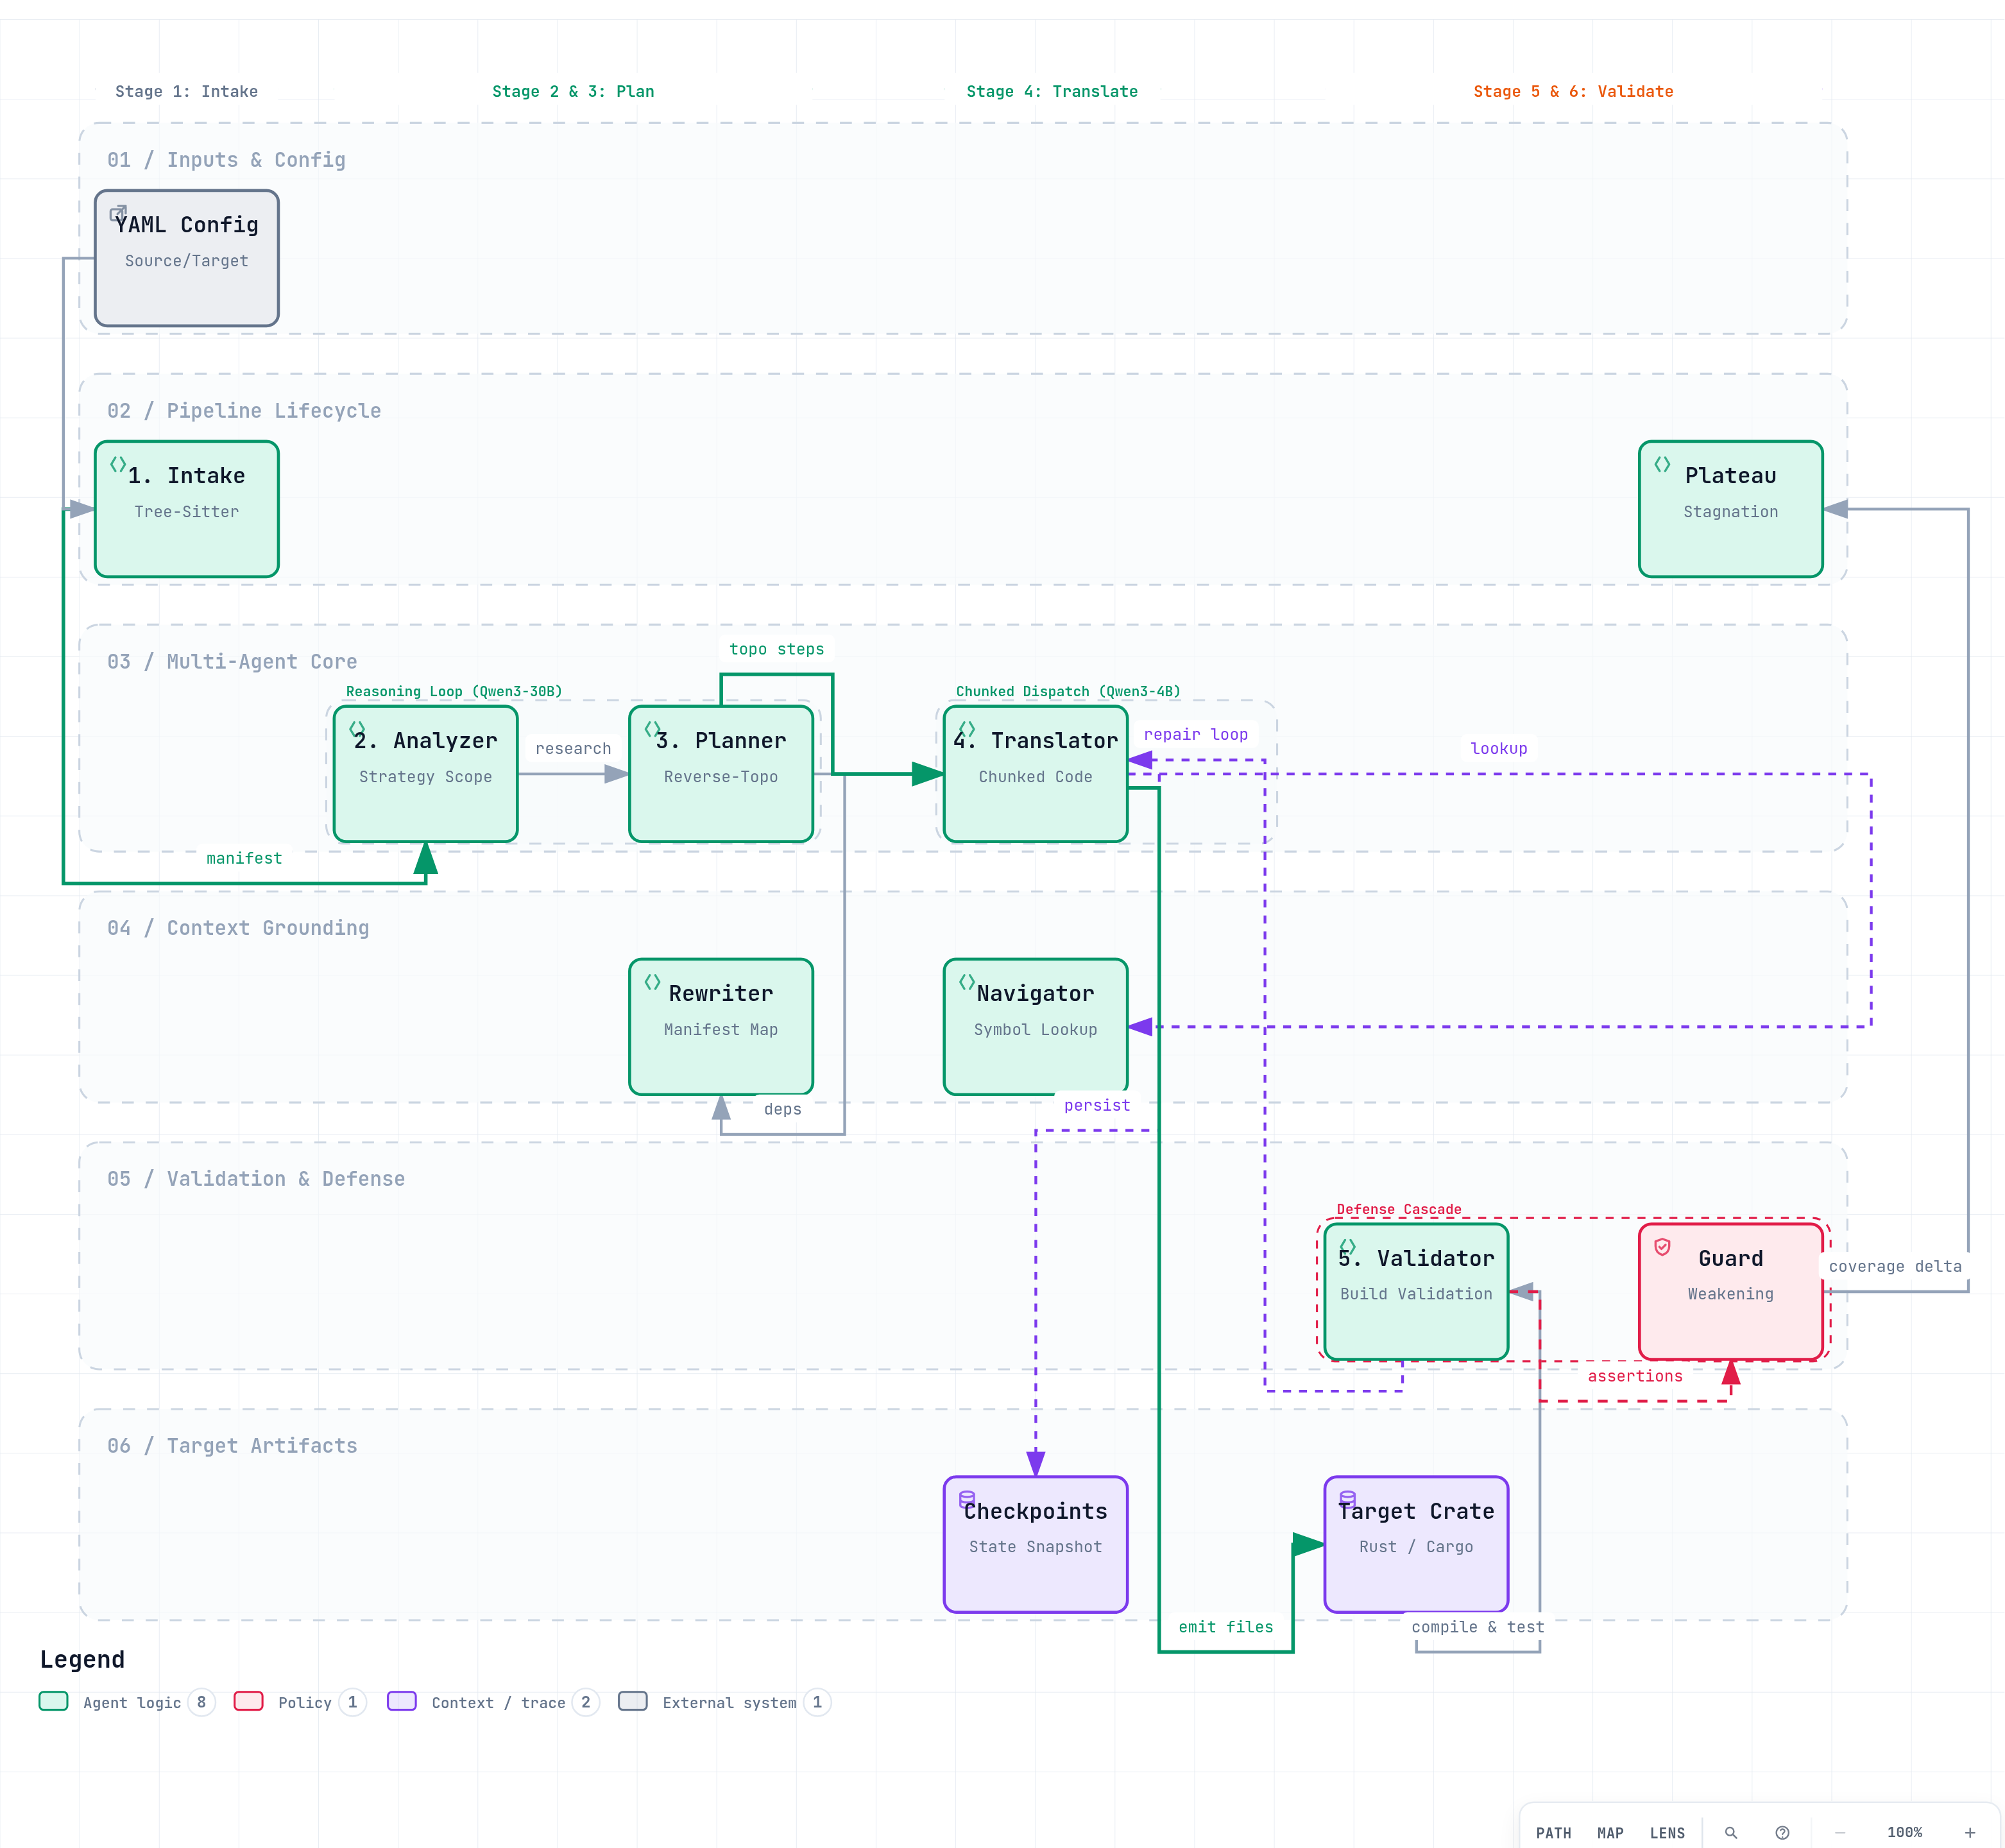
\includegraphics[width=\textwidth]{figures/fig1_workflow.png}
    \vspace{-0.5em}
    \caption{Architecture overview of the MAgHARCM multi-agent translation pipeline. The system coordinates four specialized agents: Analyzer, Planning, Translator, and Validator across an explicit six-stage execution lifecycle.}
    \label{fig:workflow}
\end{figure*}

\subsection{System Architecture Overview}
\label{sec:method_arch}

\textbf{Figure~\ref{fig:workflow}} illustrates the six execution stages of MAgHARCM. Algorithm~\ref{alg:magharcm_pipeline} outlines the end-to-end orchestration procedure with structured inputs, outputs, and validation control branches.

\begin{algorithm}[MAgHARCM Repository Translation Orchestration]
\label{alg:magharcm_pipeline}
\begin{algorithmic}[1]
\Input Source project $P_s$, Source language $L_s$, Target language $L_t$, Max iterations $K$
\Output Translated target project $P_t$
\StateIndent $G_{\text{AST}}, \text{Manifest} \gets \Call{ExtractAST}{P_s}$
\StateIndent $\mathcal{S}_{\text{strat}}, \text{Design} \gets \Call{Analyze}{G_{\text{AST}}, \text{Manifest}, L_s, L_t}$
\StateIndent $DAG, \text{Plan}, \text{Skel} \gets \Call{Plan}{G_{\text{AST}}, \text{Design}, L_s, L_t}$
\StateIndent $P_t \gets \Call{InitializeCrate}{\text{Skel}, \text{Plan}}$
\StateIndent $P_t \gets \Call{TranslateChunked}{\text{Translator}, P_t, \text{Plan}}$
\StateIndent $\Call{SaveCheckpoint}{P_t, \text{iter}=0}$
\StateIndent $\text{iter} \gets 0$
\WhileIndent{$\text{iter} < K$}
    \StateDIndent $\text{Report} \gets \text{ValidatorAgent}.\Call{Validate}{P_t, P_s}$
    \IfDIndent{$\text{Report}.\text{AllSuccess} = \text{True}$}
        \StateTIndent \Return $P_t$ \Comment{Successfully converged}
    \EndIfIndent
    \IfDIndent{$\text{Report}.\text{PlateauDetected} \lor \text{Report}.\text{Weakened}$}
        \StateTIndent \textbf{break} \Comment{Coverage plateau or security guard triggered}
    \EndIfIndent
    \StateDIndent $P_t \gets \text{TranslatorAgent}.\Call{Repair}{P_t, \text{Report}}$
    \StateDIndent $\text{iter} \gets \text{iter} + 1$
    \StateDIndent $\Call{SaveCheckpoint}{P_t, \text{iter}}$
\EndWhile
\StateIndent \Return $P_t$
\end{algorithmic}
\end{algorithm}

\subsection{Analyzer Agent \& M\"uller Strategy Selection}
\label{sec:method_analyzer}

The Analyzer Agent inspects the incoming codebase $P_s$ to build an architectural specification~\cite{p45_rajlich,p47_foltz}. Using Tree-Sitter grammars for C, Go, and Java, the agent parses the directory structure, locating module boundaries, structs, and function signatures. 

To adjust pipeline execution to repository size, the Analyzer applies M\"uller Migration Strategy Selection~\cite{muller2022towards,p46_muller_migration}. For small utility packages ($\le 5$ files and $\le 1{,}000$ LoC), the Direct Strategy translates all definitions in a single prompt. For standard multi-module repositories ($5 < |F_s| \le 50$ files or $1{,}000 < \text{LoC} \le 10{,}000$), the Incremental Strategy translates module-by-module in reverse-topological order. For enterprise codebases ($> 50$ files or $> 10{,}000$ LoC), the Pilot Strategy isolates a foundational subsystem as a self-contained pilot before expanding to remaining packages.

\subsection{Planning Agent \& Reverse-Topological DAG}
\label{sec:method_planning}

The Planning Agent converts the architectural analysis into an executable dependency schedule~\cite{p03_codeplan,p62_repograph}. A frequent failure mode in multi-file translation is caller-before-callee synthesis. If module $A$ depends on module $B$, translating $A$ first causes the model to guess type signatures for $B$, causing type mismatches when $B$ translates later.

To ensure dependencies resolve before usage, the Planning Agent builds a directed call graph $G = (V, E)$ over all extracted AST fragments~\cite{p16_code_property_graphs,p34_pdg,p35_sdg}. We compute a Reverse-Topological Order using depth-first search with back-edge removal, shown in Algorithm~\ref{alg:reverse_topo}.

\begin{algorithm}[Cycle-Free Reverse-Topological Scheduling]
\label{alg:reverse_topo}
\begin{algorithmic}[1]
\Input Directed dependency graph $G = (V, E)$
\Output Reverse-topological execution sequence $\mathcal{Q}$
\StateIndent $\text{Visited} \gets \emptyset, \quad \text{OnStack} \gets \emptyset, \quad \mathcal{Q} \gets []$
\StateIndent \Function{Visit}{$u$}
    \StateDIndent $\text{Visited} \gets \text{Visited} \cup \{u\}$
    \StateDIndent $\text{OnStack} \gets \text{OnStack} \cup \{u\}$
    \ForIndent{$(u, v) \in E$}
        \IfDIndent{$v \in \text{OnStack}$}
            \StateTIndent $E \gets E \setminus \{(u, v)\}$ \Comment{Cut cyclic back-edge}
        \ElsIfIndent{$v \notin \text{Visited}$}
            \StateTIndent \Call{Visit}{$v$}
        \EndIfIndent
    \EndForIndent
    \StateDIndent $\text{OnStack} \gets \text{OnStack} \setminus \{u\}$
    \StateDIndent $\mathcal{Q}.\Call{append}{u}$
\StateIndent \EndFunction
\ForIndent{$u \in V$}
    \IfDIndent{$u \notin \text{Visited}$}
        \StateTIndent \Call{Visit}{$u$}
    \EndIfIndent
\EndForIndent
\StateIndent \Return $\mathcal{Q}$
\end{algorithmic}
\end{algorithm}

When circular references occur (node $v$ is on the active recursion stack), the back-edge $(u, v)$ is removed from the planning DAG and recorded in the repair ledger~\cite{p02_alphatrans}. Furthermore, the Planning Agent uses a Canonical Manifest Rewriter that maps source dependencies to standard target crates in `Cargo.toml`~\cite{p58_cargo_build_system_rewriting,p60_java_maven_rust_empirical}.

\begin{figure*}[!t]
    \centering
    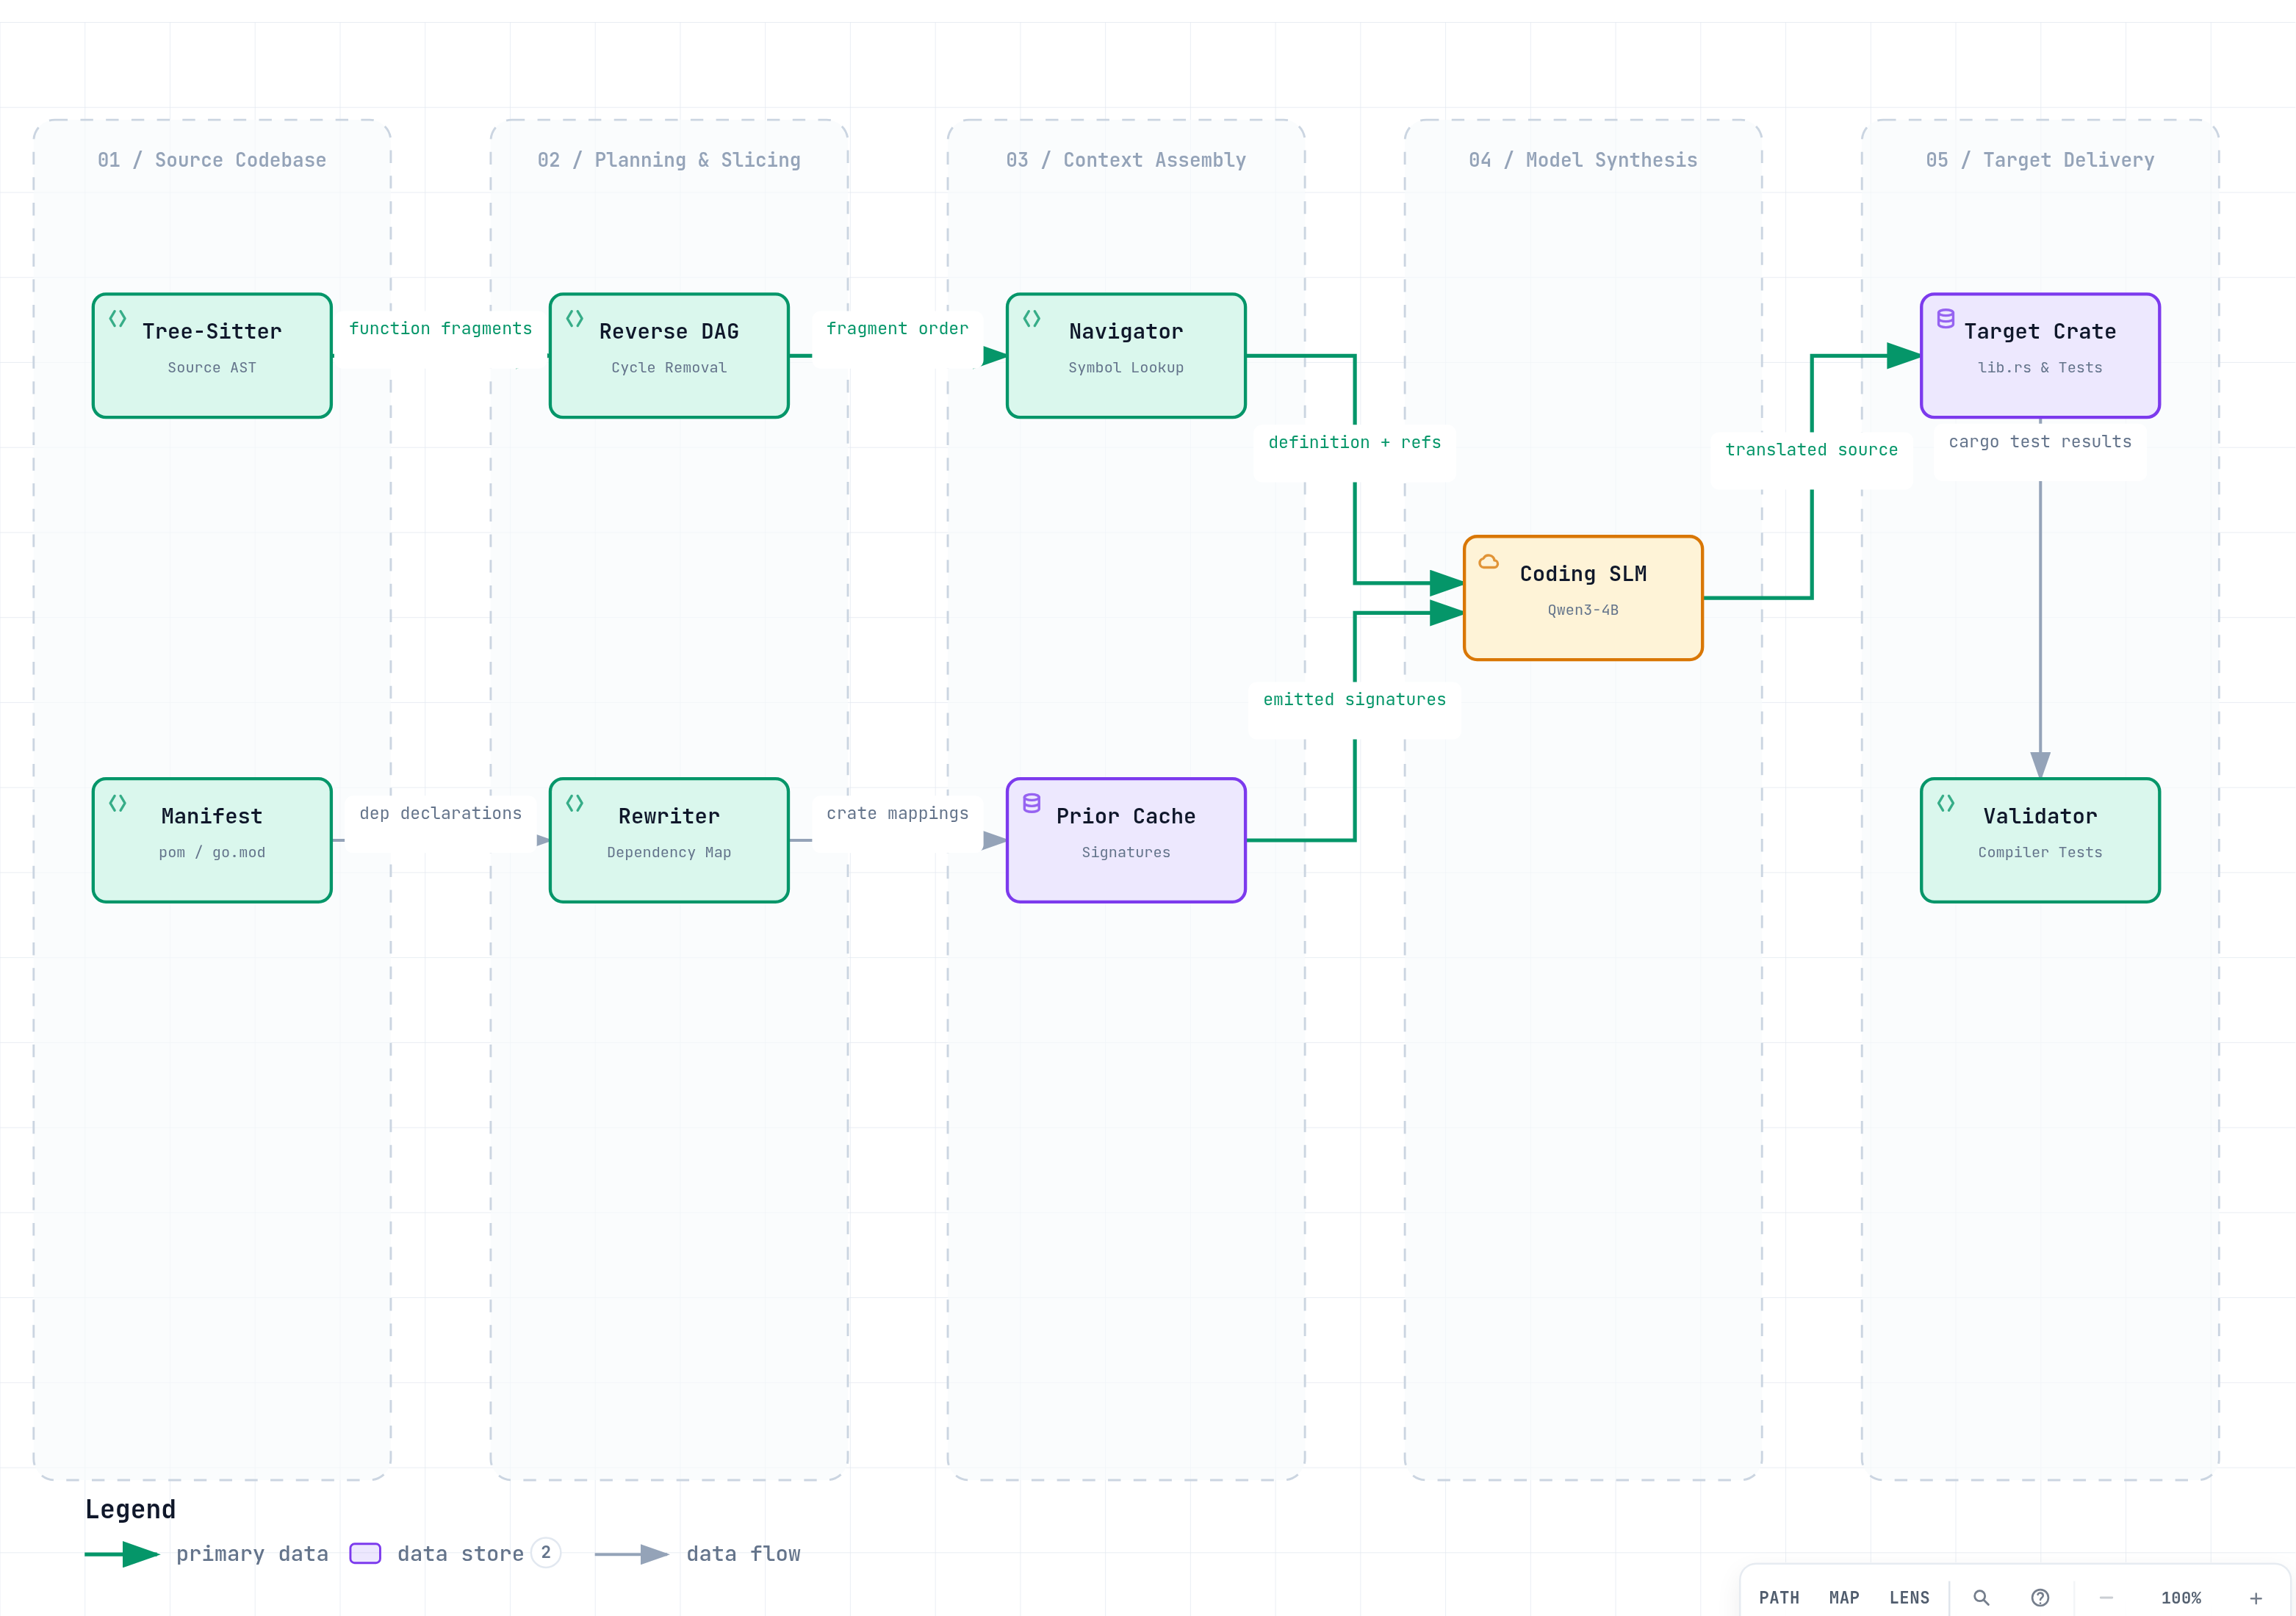
\includegraphics[width=\textwidth]{figures/fig3_dataflow.png}
    \vspace{-0.5em}
    \caption{Data flow architecture for chunked translation and context synthesis. Context bounds are capped at $\le 4$\,KB via the Symbol Navigator and Prior Memory to avoid local SLM context saturation.}
    \label{fig:dataflow}
\end{figure*}

\subsection{Translator Agent \& Chunked Context Synthesis}
\label{sec:method_translator}

The Translator Agent emits target code from planning fragments. To operate reliably on local 4B--7B coding models, the Translator uses Chunked Translation as depicted in \textbf{Figure~\ref{fig:dataflow}}. Instead of transmitting the entire repository, the agent processes one module fragment at a time.

Context assembly uses two mechanisms. First, the Symbol-Aware Navigator provides relevant upstream struct definitions, function signatures, and trait bounds within a compact $\le 4$\,KB context window~\cite{p13_hyperagent,p61_repocoder}. Second, the Prior-Modules Memory maintains a running summary ($\le 4$\,KB) of already emitted module paths and exported signatures. This ensures newly generated modules import and reuse existing types consistently.

\begin{figure*}[!t]
    \centering
    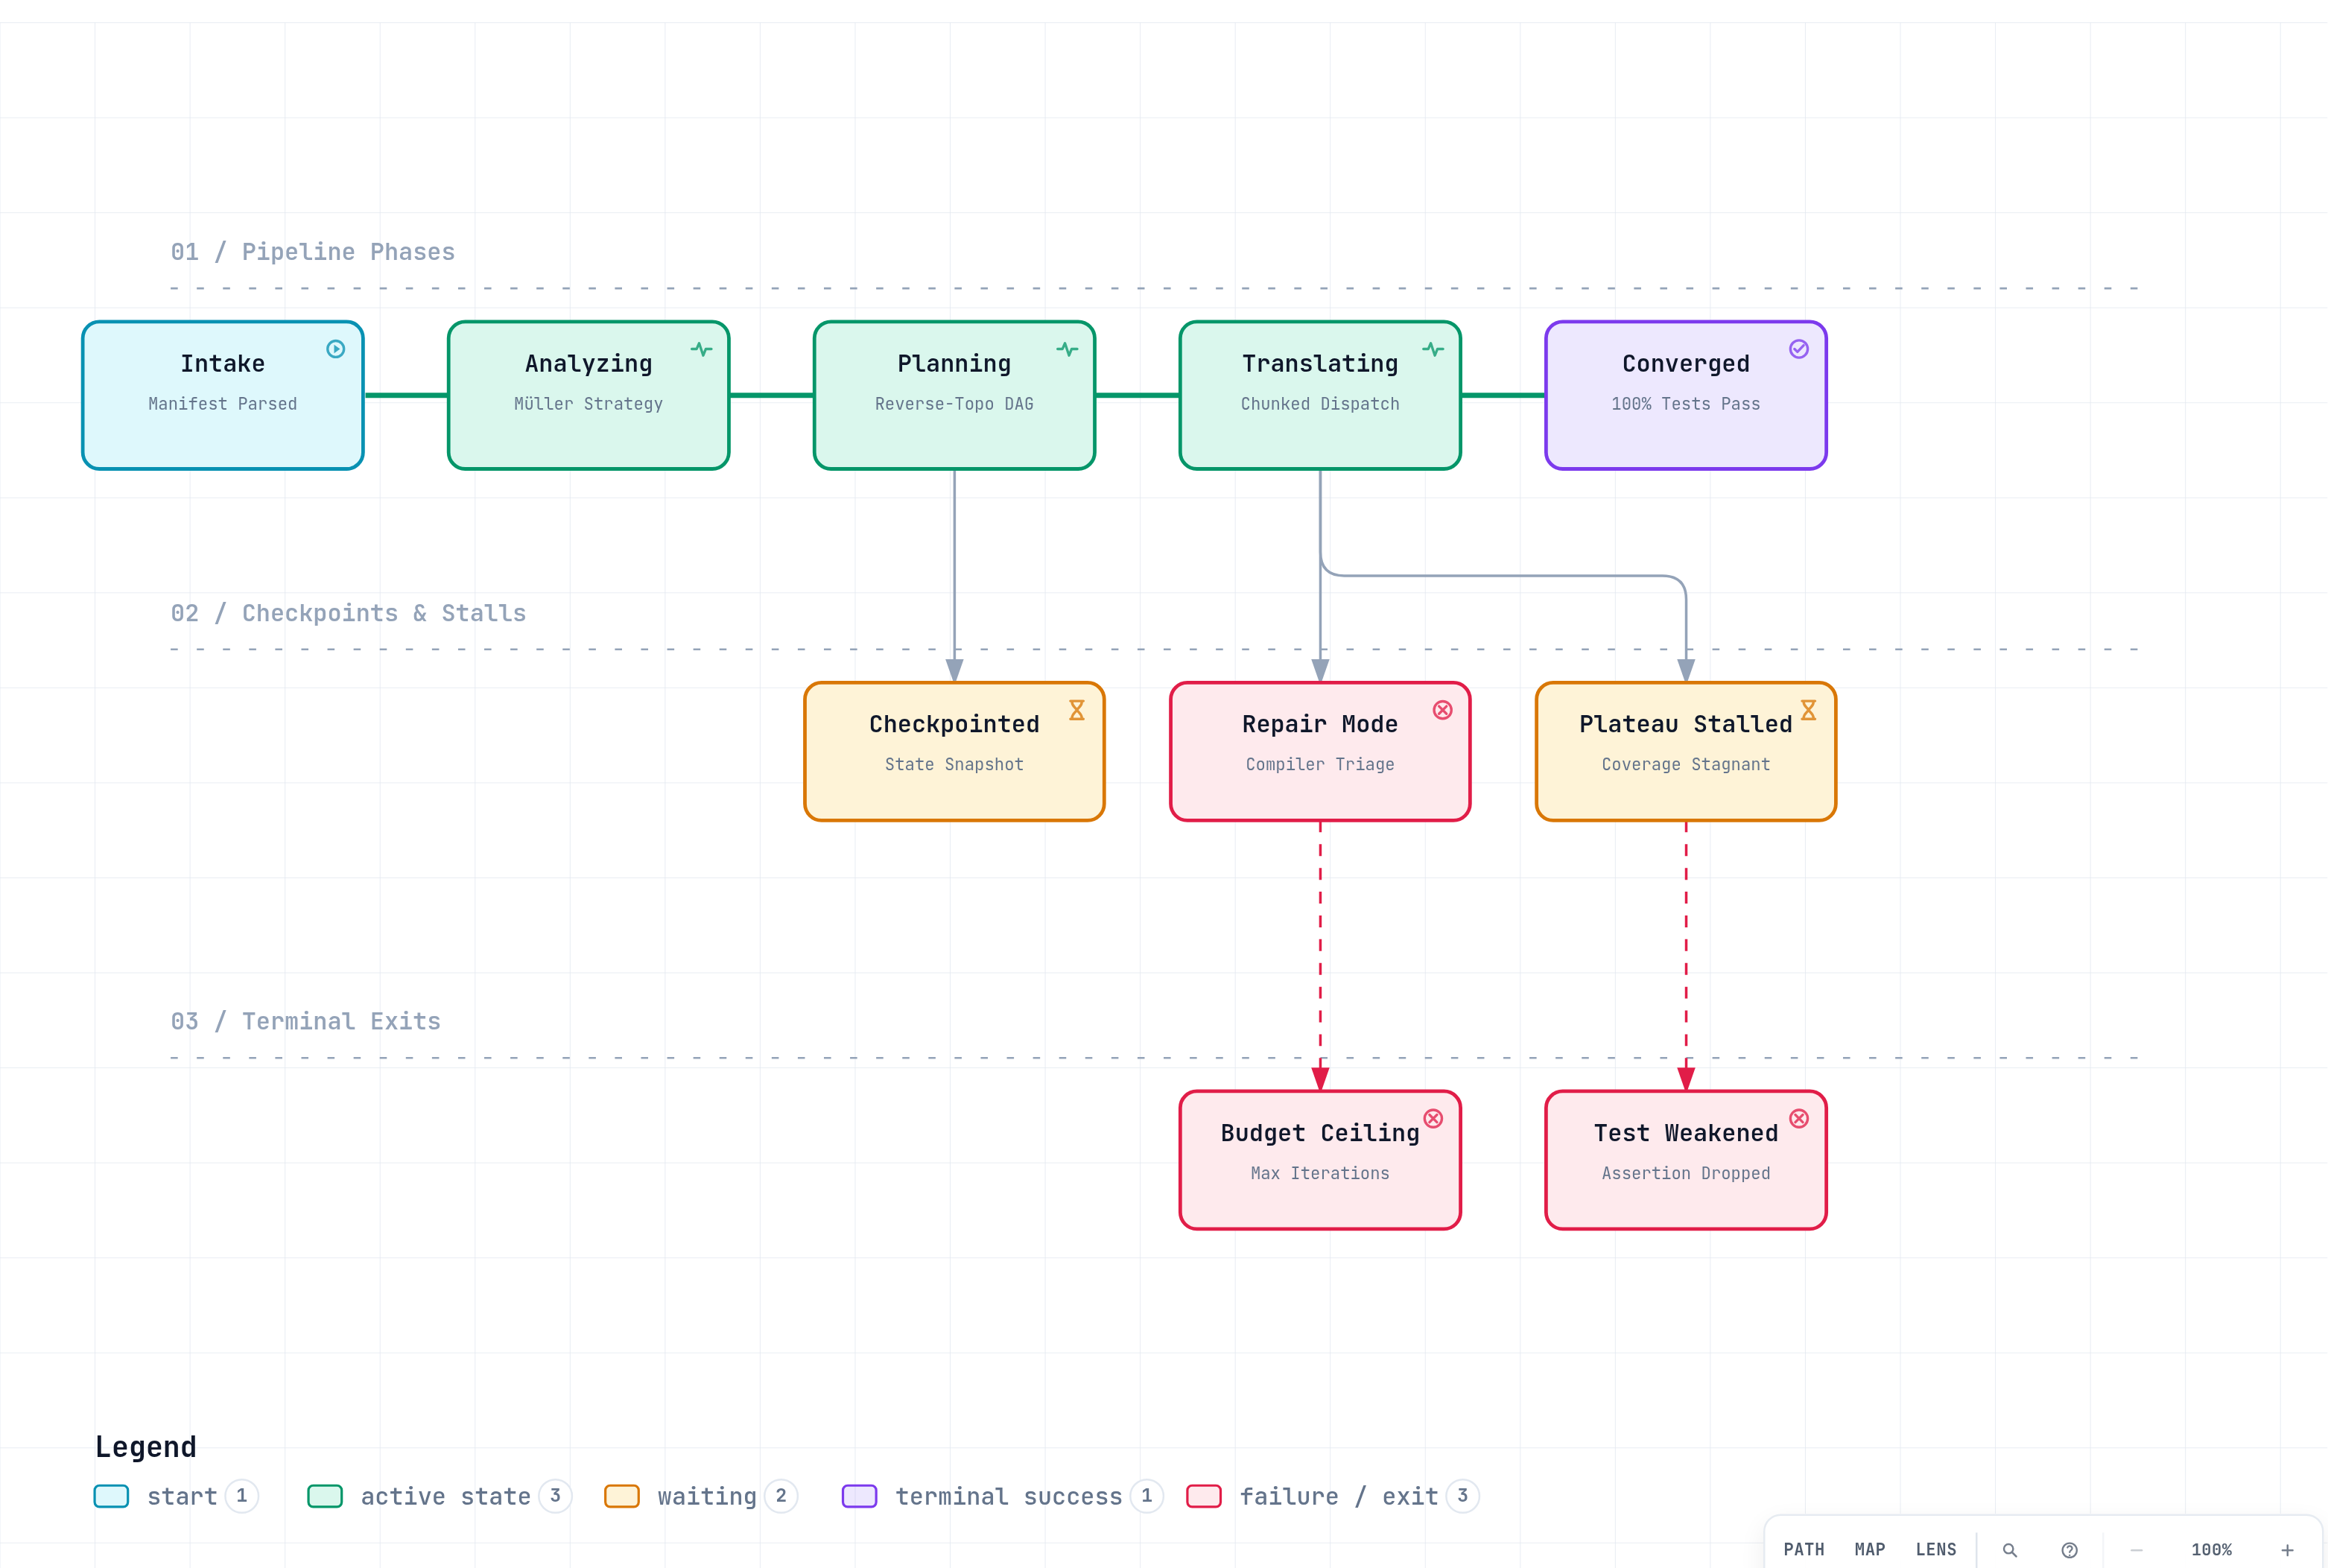
\includegraphics[width=\textwidth]{figures/fig4_lifecycle.png}
    \vspace{-0.5em}
    \caption{State machine lifecycle of MAgHARCM. The system tracks states across intake, analysis, planning, chunked translation, test validation, checkpoints, and multi-stage repair.}
    \label{fig:lifecycle}
\end{figure*}

\subsection{Validator Agent \& Multi-Stage Defense Cascade}
\label{sec:method_validator}

The Validator Agent verifies target code quality and enforces functional correctness. \textbf{Figure~\ref{fig:lifecycle}} depicts the complete state machine lifecycle of the verification and repair process.

The validation cascade includes five checks. The AST Syntax Pre-Check validates target source files using Tree-Sitter before running the compiler toolchain. The Native Toolchain Build Validation executes `cargo check` or `cargo test --no-run` to capture compiler diagnostics and borrow-checker errors ($E0382, E0502$). The Test Suite Execution runs target unit tests and records passing assertion counts~\cite{p20_evosuite,p23_pynguin}. The Adversarial Weakening Guard compares test AST assertions between iterations, preventing repair passes from deleting assertions or relaxing equality checks~\cite{p25_advtestgen,p08_matchfixagent}. Finally, the Coverage Plateau Detector adapts CodaMOSA search stagnation logic~\cite{p49_codamosa,lemieux2023codamosa} to track test gains across iterations, halting execution gracefully if repair rounds produce zero progress.
